
{\actuality}
\ifsynopsis
Задачи термоупругости возникают в самых разных областях инженерного дела: аэрокосмической отрасли, строительстве, микроэлектронике и многих других. Передовые технологии таких отраслей, как правило, тесно связаны с созданием новых материалов. При этом часто требования уже настолько высоки, что при их создании необходимо учитывать молекулярную структуру материала, напрямую влияющую на свойства среды. Такие материалы принято называть структурно-чувствительными.
\else
Задачи термоупругости очень популярны в различных инженерных приложениях, так как температурные деформации могут существенным образом повлиять на функциональные свойста рассматриваемых объектов, вплоть до их полного выхода из строя. Особенно популярны такого рода задачи в аэрокосмической отрасли при моделировании поведения обшивок корпусов и двигателей летательных аппаратов \cite{Aerocosmos1, Aerocosmos2, Aerocosmos3}, так как они подвержены очень высоким и в то же время неравномерным нагружениям \cite{Aerocosmos4, Aerocosmos5, Aerocosmos6, Aerocosmos7}. Помимо аэрокосмической отрасли такие задачи могут быть востребованы в строительстве, особенно в строительстве критической инфраструктуры, такой, например, как атомные электространции \cite{StroyMech1, StroyMech2}. В гражданской инфраструктуре актуален анализ влияния таких разрушительных явлений как пожары \cite{StroyMech3, StroyMech4} или обычная циклическая смена сезона \cite{StroyMech5, StroyMech6}, при воздействии которых конструкция не должна потерять устойчивость. В микроэлектронике эти задачи также не остаются без внимания \cite{MicroElectronic1, MicroElectronic2}, а учитывая возрастающее количество вычислительных мощностей и популярность микро- и наноэлектромеханических систем (МЭМС/НЭМС), возникают задачи об эффективном отводе тепловой энергии~\cite{MicroElectronic3}.
\fi

\ifsynopsis
Важным этапом в создании новых материалов является построение математической модели, способной адекватно описывать их поведение. Классические материалы можно описать моделями механики сплошной среды, однако, когда речь идет о структурно-чувствительных материалах, где величина структуры не превышает нескольких десятков нанометров, гипотеза сплошности нарушается, из-за чего приходится прибегать к другим моделям, например, моделям молекулярной динамики или статистическим моделям. Анализ такого рода моделей очень ограничен без численного эксперимента, а для проведения полноценного эксперимента необходимы большие вычислительные мощности, которые не всегда доступны исследователю. В связи с этим в середине XX века набирают популярность модели обобщённой механики сплошной среды, которые могут учесть такие явления, как микровращения отдельных зёрен материала, микродислокации, различные дальнодействующие и многие другие масштабные эффекты.
\else
Все перечисленные ранее и многие другие задачи объединяет потребность в создании новых материалов, которые будут отвечать соответствующим их использованию требованиям. На сегодняшний день в некоторых отраслях требования к свойствам материалов становятся уже настолько высокими, что при их создании необходимо учитывать молекулярную структуру материала на микро- и наноуровне \cite{MaterialStructure1, MaterialStructure2, MaterialStructure3}, так как их свойства могут напрямую зависеть от этого. Такие материалы принято называть структурно-чувствительными, а создание материалов с наперёд заданными свойствами на сегодняшний день является одной из сложнейших, но вместе с этим крайне актуальной областью материаловедения \cite{Auxetics}.
\fi

\ifsynopsis
В диссертационной работе рассмотрен класс моделей, обеспечивающих описание дальнодействующих эффектов путём обобщения классических уравнений механики сплошной среды и представлении их в интегро-дифференциальной форме. Такие модели принято называть нелокальными, а их разработка активно велась в рамках работ следующего списка авторов: E.~Kr{\"o}ner, D.G.B.~Edelen, A.C.~Eringen, D.~Rogula, S.B.~Altan, C.~Polizzotto, A.A.~Pisano, В.В.~Васильев, С.А.~Лурье, С.Л.~Соболев, В.С.~Зарубин, Г.Н.~Кувыркин, И.Ю.~Савельева и многие другие.
\else
Вместе с проблемой создания структурно-чувствительных материалов многие исследователи сталкиваются с проблемой моделирования их поведения. При рассмотрении наномасштабных структур отсутствует возможность использовать гипотезу сплошности среды, из-за чего классические модели механики сплошной среды не могут даже на качественном уровне передать все особенности их поведения. Так, например, в наномасштабе перестаёт работать гипотеза Био --- Фурье \cite{FourierLaw1, FourierLaw2} и наблюдается пониженная чувствительность к концентраторам напряжений \cite{ConcentrationInsensitive1, ConcentrationInsensitive2}. Этому способствуют такие эффекты, как микровращения отдельных зёрен материала, микродислокации, различные дальнодействующие и многие другие масштабные эффекты, которые могут быть смоделированы только при помощи новых математических моделей.
\fi

\ifsynopsis
В практических приложениях на основе математической модели необходимо решать большую серию задач, не все из них обладают аналитическими решениями. В связи с этим необходимо развивать подходы с использованием численных методов решения уравнений с последующей реализацией в виде программного комплекса. В диссертационной работе этому аспекту уделено особое внимание. За основу численной схемы был взят метод конечных элементов, его реализация стала частью программного комплекса NonLocFEM.
\nocite{AMCSM2019}
		\nocite{ZAMM}
		\nocite{NonlocalSaintVenant}
		\nocite{NonlocalRadiation}
\else
На сегодняшний день существует большое количество моделей способных описать различные масштабные эффекты. Однако подходы моделирования могут достаточно сильно различаться между собой при рассмотрении разных линейных размеров и временных отрезков. Таким образом, возникают иерархии моделей, способных качественно и количественно описать различные аспекты поведения материала на разных масштабах. Это, в свою очередь, приводит к идее многомасштабного моделирования \cite{Multiscale1}, где, например, некоторые характеристики материала можно вычислять при помощи моделей, находящихся ниже по иерархии, и передавать полученные в расчётах параметры в вышестоящие модели или наоборот.
\fi

\ifsynopsis
\else
Для механики твёрдого тела одна из возможных иерархий моделей проиллюстрирована на Рис. \ref{fig:ModelsHierarchy}. Согласно такому представлению модели, использующие аппарат квантовой механики \cite{QuantumModelling1, QuantumModelling2}, находятся на первой ступени иерархии, их применение ограничено масштабами сопоставимыми с ядрами атомов и простейших молекулярных соединений, состоящих из небольшого числа атомов, то есть в диапазоне от нескольких ангстрем до нескольких нанометров. На второй ступени иерархии находятся модели молекулярной динамики \cite{MD1, MD2, MD3, MD4}, такие модели могут описывать поведение сложных соединений, например, больших полимерных молекул и прочих наномасштабных объектов, размеры которых не превосходят нескольких десятков нанометров. На третьей ступени располагаются статистические модели, в частности модели, в основе которых лежит метод Монте-Карло \cite{MonteCarlo1, MonteCarlo2}. В таких моделях расчёты проводят многократно, а структуру рассматриваемого объекта генерируют случайным образом по определённым правилам, после чего полученные таким способом результаты осредняют или вычисляют на их основе вероятностные характеристики материала. И на последней --- четвёртой ступени иерархии стоят континуальные модели, в частности модели механики сплошной среды \cite{MSS}. Такие модели оперируют гипотезами сплошности среды и абсолютности времени, то есть не учитывают дискретность рассматриваемого вещества.
\fi

\ifsynopsis
\else
\begin{figure}[ht]
    \centerfloat{
        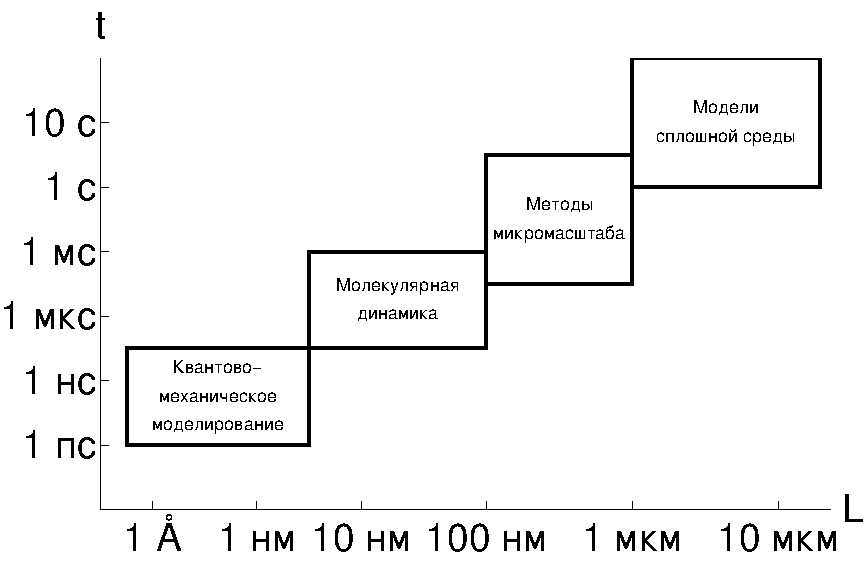
\includegraphics[width=0.85\textwidth]{pics/ModelsHierarchy.pdf}
    }
    \caption{Иерархия моделей}\label{fig:ModelsHierarchy}
\end{figure}
\fi

\ifsynopsis
\else
Однако у статистических моделей и моделей молекулярной динамики есть недостаток --- анализ объектов при помощи этих моделей без численных экспериментов крайне ограничен \cite{MDExperiment}. Поэтому с середины XX века набирают популярность модели обобщённой механики сплошной среды, которые распространяют применение моделей высшего уровня на области применения моделей низшего уровня. Одна из первых таких моделей была предложена в работе братьев Eugène и François Cosserat \cite{Cosserat}, где помимо трансляционных степеней свободы также были учтены и вращательные компоненты движения, которые связаны с трансляционными рядом соотношений, из-за чего тензор напряжений перестаёт быть симметричным. Позже, спустя пол века, эта теория была связана с теорией дислокаций в работе V.~G{\"u}nther \cite{CosseratAndDislocation} и дополнена законом сохранения микроинерции в работе A.C.~Eringen \cite{Eringen2, Eringen3}, в связи с чем теорию начали называть микрополярной теорией упругости. Также к работам, в которых исследована микрополярная теория упругости, можно отнести работы R.D.~Mindlin \cite{Mindlin1, Mindlin2, Mindlin3}, D.B.~Bogy \cite{Bogy} и Y.C.~Hsu \cite{Hsu}. В них авторы рассматривали применение этой теории в задачах с концентраторами, возникающим в углах и отверстиях соответсвенно. В то же время теория нашла своё отражение в работах советских учёных Э.Л.~Аэро и Е.В.~Кувшинского \cite{Aero1,Aero2}, а также была рассмотрена в работах Н.Ф.~Морозова \cite{Morozov} и Г.Н.~Савина \cite{Savin}.
\fi

\ifsynopsis
\else
Дальнейшее развитие микрополярной теории упругости привело к появлению микроморфных моделей \cite{Eringen4, Micromorph1, Micromorph2}, в которые помимо вращательных компонент движения могут быть включены дополнительные переменные, связанные с деформацией материала, при этом микрополярная теория упругости является лишь частным случаем микроморфных моделей. Но стоит учесть тот факт, что использование таких моделей сопряжено с трудностью определения материальных коэффициентов.
\fi

\ifsynopsis
\else
Список рассмотренных моделей, учитывающих микровращение, а также авторов, которые занимались их развитием и исследованием, далеко не исчерпывающий. Однако стоит также уделить внимание другому классу моделей обобщённой механики сплошной среды, описывающих дальнодействующие эффекты. Это градиентные модели, которые получили своё развитие в 60-х годах XX века. Эти модели оперируют высшими производными деформаций, в связи с чем они и получили такое название. Первые модели градиентной теории упругости были сформулированы в работах Toupin~R.A. \cite{Toupin} и Mindlin~R.D. \cite{Mindlin4, Mindlin5}, которые сейчас в литературе принято называть моделями Миндлина --- Тупина \cite{ToupinMindlin1, ToupinMindlin2, ToupinMindlin3}. В работе G.~Ahmadi и K.~Firoozbakhsh \cite{GradientThermoelasticity} эти модели получили обобщение на температурные деформации. Как и микроморфные, градиентные модели обладают тем же недостатком --- большое количество материальных констант, которые необходимо определить, поэтому в 90-х годах XX века в работах E.C.~Aifantis и его соавторов \cite{Aifantis1, Aifantis2} была рассмотренна упрощёная модель градиентной теории упругости, в которой напряжения связаны с деформацией и её вторым градиентом, и, по сравнению с классической моделью, был добавлен всего один дополнительный материальный параметр внутренней длины.
\fi

\ifsynopsis
\else
Существует ещё один класс моделей, описывающих дальнодействующие эффекты, --- это нелокальные модели, которые в отличие от градиентных оперируют интегральными выражениями типа свёртки. Впервые описание таких моделей было представлено в работе E.~Kr{\"o}ner \cite{Kroner}, где были рассмотрены упругие среды с дальнодействующими силами сцепления. Модели нелокальной упругости в термодинамическом контексте были рассмотрены в работах D.G.B.~Edelen, A.E.~Green и N.~Laws \cite{Edelen1, Edelen2}, позже к их работе присоединился и A.C.~Eringen \cite{Eringen5, Eringen6}. Исследование условий, обеспечивающих существование фундаментальных решений было проведено в работе D.~Rogula \cite{Rogula1982}. Вопросы, связанные с существованием и единственностью решений начально-краевых задач теории нелокальной упругости были рассмотрены в работах S.B.~Altan \mbox{\cite{Altan1, Altan2},} позже он рассмотрел этот вопрос и для задач нелокальной термоупругости \mbox{\cite{Altan3, Altan4}.} В конечном итоге, в начале XXI века, A.C.~Eringen представил работу \cite{Eringen1}, в которой описан единый подход к построению нелокальных теорий для упругих тел, в связи с чем в литературе нелокальные модели часто называют моделями Эрингена и их исследованию посвящено достаточно большое количество работ \cite{BondaryLayer, Tuna, Rahmani}. При этом между нелокальными и градиентными моделями существует связь, которая была рассмотрена в работах S.B.~Altan и E.C.~Aifantis \cite{Aifantis3}, J.~Gao \cite{Gao} и др.
\fi

\ifsynopsis
\else
У нелокальных моделей также есть свои недостатки. Главный из них~--- необходимость введения дополнительных условий, так как обычных граничных условий будет недостаточно \cite{Pisano2}. Поэтому в прикладных исследованиях используют регуляризованные модели, в которых рассматривают комбинированные среды, состоящие из локальной и нелокальной фаз. Первые примеры рассмотрения такого рода сред можно найти в работах C.~Polizzoto \cite{Polizzotto1, Polizzotto2}, где были проанализированы одномерные задачи упругости, а также разработан численный метод решения на основе метода конечных элементов. Развитие этих идей в рамках двумерных задач нелокальной упругости было описано в работе A.A.~Pisano~\cite{Pisano1}.
\fi

\ifsynopsis
\else
Анализ моделей нелокальной телопроводности на примере решения одномерных задач был проведён в работе Г.Н.~Кувыркина и И.Ю.~Савельевой~\cite{NonlocalThermal1}. В это же время Г.Н.~Кувыркином были рассмотрены нелокальные модели термовязкоупругости в работах \cite{ThermoViscoElasticity1, ThermoViscoElasticity2, ThermoViscoElasticity3}. Позже в работах И.Ю.~Савельевой были рассмотрены задачи термоудара \cite{ThermoUdar1, ThermoUdar2} и вариационные постановки задачи \cite{NonlocalThermalVariation1, NonlocalThermalVariation2}. Наиболее общий представлены в работе \cite{SavelievaDisser}. К исследованиям нелокальных моделей были подключены и ученики Г.Н.~Кувыркина в том числе и автор данной диссертационной работы~\mbox{\cite{AMCSM2019, ZAMM, NonlocalSaintVenant, NonlocalRadiation, KirshProblem}.}
\fi

\ifsynopsis
\else
Решение задач в нелокальных постановках вызывает достаточно много сложностей, так как приходится иметь дело с интегро-дифференциальными уравнениями, которые не всегда имеют аналитические решения даже на простых областях. В этом случае необходимо использовать различные численные методы, специально адаптированные под данный класс уравнений. В этом направлении есть уже достаточно большое количество работ, предлагающих использовать различные методы решения. Наиболее общим и популярным является метод конечных элементов (FEM), который применительно к данному классу уравнений иногда ещё называют методом нелокальных конечных элементов (NL-FEM) \cite{Polizzotto2, Pisano1}. Однако его использование сопряжёно с большой вычислительной сложностью. Поэтому некоторые исследователи используют его модификацию на основе быстрого преобразования Гаусса (FEMFGT) \cite{FastGaussTransform}. Но использование такого подхода сопряжено с проблемами контроля точности. Для того, чтобы избежать осциляций, необходимо решать задачи на достаточно подробных сетках, что в некоторых ситуациях лишает данный подход ожидаемых преимуществ перед прямым методом решения. Помимо сеточных методов большой популярностью пользуются и бессеточные подходы на основе радиальных базисных функций \cite{RadialBasis}, безэлементный метод Галёркина (EFG) и метод конечных точек (FPM) \cite{MeshFree}. Также были предложены подходы с использованием пограничного слоя \cite{BondaryLayer} и на основе полиномов Чебышёва \cite{ChebPolynom}, однако на практике этот метод не применяется в силу своей трудоёмкости, но он может быть использован для оценки качества решения другими методами.
\fi

\ifsynopsis
\else
В рамках текущей работы было принято решение использовать метод нелокальных конечных элементов, так как данный метод достаточно хорошо изучен и его легко использовать на областях со сложной геометрией, а большое количество редакторов и генераторов сеток упрощает процесс моделирования. Также в работе проведена большая работа по ускорению данного метода, но чтобы в полной мере реализовать весь потенциал предложенных алгоритмов был реализован свой собственный програмный комплекс NonLocFEM \cite{NonLocFEM} на языке программирования C++. Такое решение связано с тем, что многие современные коммерческие программные комплексы, например Abaqus~\cite{Abaqus}, Ansys~\cite{Ansys}, TFlex~\cite{TFlex} и др., имеют закрытый программный код. С другой стороны существуют открытые программные комплексы, например, Deal.II~\cite{DealII}, FEniCS~\cite{FEniCS}, FreeFEM~\cite{FreeFEM} и многие другие. Однако использование открытых программных комплексов так же может повлечь за собой определённый ряд проблем. Например, одной из проблем может стать невозможность эффективно реализовать тот или иной алгоритм в силу базовых принципов, которые заложены в программный комплекс. Вторая, наверное даже более серьёзная проблема, связана с потенциальным конфликтом интересов, так как многие программные комплексы созданы при поддержке зарубежных инвесторов, которые в любой момент могут ограничить к ним доступ и поэтому важно иметь собственные отечественные наработки.
\fi

%\ifsynopsis
%Этот абзац появляется только в~автореферате.
%\else
%Этот абзац появляется только в~диссертации.
%\fi

% {\progress}
% Этот раздел должен быть отдельным структурным элементом по
% ГОСТ, но он, как правило, включается в описание актуальности
% темы. Нужен он отдельным структурынм элемементом или нет ---
% смотрите другие диссертации вашего совета, скорее всего не нужен.

{\aim} исследования является изучение особенностей разработанных двумерных моделей нелокальной теплопроводности и термоупругости, а также сравнительный анализ решений в случае классических и нелокальных моделей механики сплошной среды.

Для достижения поставленной цели потребовалось решить {\tasks}.
\ifsynopsis

1. Разработать определяющие соотношения двумерных моделей теплопроводности и термоупругости нелокальной среды в интегро-дифференциальной форме, а также реализовать эффективные алгоритмы численного решения на основе метода конечных элементов с последующей реализацией в виде собственного программного комплекса.

2. Разработать экономичные способы предобуславливания получаемых при аппроксимации систем линейных алгебраических уравнений (СЛАУ) с целью ускорения сходимости итерационных методов решения.

3. Исследовать особенности нелокальных моделей, сопоставить полученные результаты в задачах с известными решениями в классической постановке, определить закономерности.
\else
\begin{enumerate}[beginpenalty=10000] % https://tex.stackexchange.com/a/476052/104425
  \item Разработать определяющие соотношения двумерных моделей теплопроводности и термоупругости нелокальной среды в интегро-дифференциальной форме, а также реализовать эффективные алгоритмы численного решения на основе метода конечных элементов с последующей реализацией в виде собственного программного комплекса.
  \item Разработать экономичные способы предобуславливания получаемых при аппроксимации систем линейных алгебраических уравнений (СЛАУ) с целью ускорения сходимости итерационных методов решения.
  \item Исследовать особенности нелокальных моделей, сопоставить полученные результаты в задачах с известными решениями в классической постановке, определить закономерности.
\end{enumerate}
\fi


{\novelty}
\ifsynopsis

1. Предложены новые эффективные численные алгоритмы для задач нелокальной теплопроводности и нелокальной термоупругости на основе метода конечных элементов, которые обладают хорошей масштабируемостью и предназначены для вычислений на многопроцессорных вычислительных машинах с общей и распределённой памятью.

2. Разработан собственный программный комплекс NonLocFEM, в котором реализованы все представленные в работе алгоритмы и методы для моделирования поведения структурно-чувствительных материалов.

3. Получены новые результаты в задачах с известными для классической постановки решениями, установлены закономерности, свидетельствующие о снижении роли концентраторов в распределениях полей напряжений и плотности теплового потока.

4. Исследованы границы спектров собственных чисел матриц и установлены связи между спектрами матриц, ассемблированных в классической и нелокальной постановках.
\else
\begin{enumerate}[beginpenalty=10000] % https://tex.stackexchange.com/a/476052/104425
  \item Предложены новые эффективные численные алгоритмы для задач нелокальной теплопроводности и нелокальной термоупругости на основе метода конечных элементов, которые обладают хорошей масштабируемостью и предназначены для вычислений на многопроцессорных вычислительных машинах с общей и распределённой памятью.
  \item Разработан собственный программный комплекс NonLocFEM, в котором реализованы все представленные в работе алгоритмы и методы для моделирования поведения структурно-чувствительных материалов.
  \item Получены новые результаты в задачах с известными для классической постановки решениями, установлены закономерности, свидетельствующие о снижении роли концентраторов в распределениях полей напряжений и плотности теплового потока.
  %\item Проведено качественное сравнение между результатами полученными с использованием классической и нелокальной теориями, которые свидетельствуют о снижении роли концентраторов в распределениях полей напряжений и плотности теплового потока.
  \item Исследованы границы спектров собственных чисел матриц и установлены связи между спектрами матриц, ассемблированных в классической и нелокальной постановках.
\end{enumerate}
\fi

{\influence}
моделей, рассмотренных в диссертации, состоит в возможности описания поведения термомеханических состояний структурно-чувствительных материалов. Параметры модели очевидным образом влияют на решения, что дает возможность точно настраивать модель для применения на практике. Разработанный программный комплекс, в котором реализованы численные алгоритмы исследования разработанных моделей, позволит проводить расчёты на произвольных областях со всеми рассматриваемыми в моделе параметрами, а благодаря открытому исходному коду и модульной структуре существует возможность редактировать существующие постановки и добавлять новые типы расчётов при модификации математической модели.

{\methods}
В диссертации использованы как классические принципы механики деформируемого твёрдого тела, так и новые, относящиеся к нелокальным теориям теплопроводности и термоупругости, а также численные методы, в основе которых лежит метод конечных элементов.

\ifsynopsis
{\defpositions}
\begin{enumerate}[beginpenalty=10000] % https://tex.stackexchange.com/a/476052/104425
 	\item Модели нелокальной теплопроводности и термоупругости, позво-
\end{enumerate}
ляющие описать процессы передачи теплоты и напряжённо-деформированного состояния в структурно-чувствительных материалах.

2. Новые численные алгоритмы решения на основе метода конечных элементов, адапатированные под многопроцессорные вычислительные системы.

3. Собственный программный комплекс NonLocFEM, в рамках которого реализованы все рассматриваемые в работе методы решений.
\else
{\defpositions}
\begin{enumerate}[beginpenalty=10000] % https://tex.stackexchange.com/a/476052/104425
 	\item Модели нелокальной теплопроводности и термоупругости, позволяющие описать процессы передачи теплоты и напряжённо-деформированного состояния в структурно-чувствительных материалах.
	\item Новые численные алгоритмы решения на основе метода конечных элементов, адапатированные под многопроцессорные вычислительные системы.
	\item Собственный программный комплекс NonLocFEM, в рамках которого реализованы все рассматриваемые в работе методы решений.
\end{enumerate}
\fi

{\reliability} результатов гарантирована строгостью и полнотой использования возможностей математического аппарата, сравнением результатов многочисленных проведеннных расчетов с известными аналитическими решениями и данными, полученными ранее другими авторами.
%{\reliability} полученных результатов гарантирует строгость используемого математического аппарата, сравнение расчётов с известными аналитическими решениями и данными полученными ранее другими авторами.

\ifsynopsis
{\probation} проводилась в обсуждениях на следующих конференциях:
Международная научно-техническая конференция <<Актуальные проблемы прикладной математики, информатикии и механики>> (Воронеж, 2019, 2021); Международная конференция <<International Conference of Numerical Analysis and Applied Mathematics>> (Родос, Греция, 2021); Международная научная конференция <<Фундаментальные и Прикладные Задачи Механики>> (Москва, 2021); Всероссийская конференция по численным методам решения задач теории упругости и пластичности (Красноярск, 2023); Международная конференция <<Математическое моделирование, численные методы и инженерное программное обеспечение>> (Москва, 2023).
\else
{\probation} проводилась в обсуждениях на следующих конференциях:
\begin{enumerate}
	\item Международная научно-техническая конференция <<Актуальные проблемы прикладной математики, информатикии и механики>> (Воронеж, 2019, 2021);
	\item Международная конференция <<International Conference of Numerical Analysis and Applied Mathematics>> (Родос, Греция, 2021);
	\item Международная научная конференция <<Фундаментальные и Прикладные Задачи Механики>> (Москва, 2021);
	\item Всероссийская конференция по численным методам решения задач теории упругости и пластичности (Красноярск, 2023);
	\item Международная конференция <<Математическое моделирование, численные методы и инженерное программное обеспечение>> (Москва, 2023).
\end{enumerate}
\fi

\ifsynopsis
Тема диссертации согласована с тематикой грантов, выделенных на фундаментальные исследования: 0705-2020-0047 <<Теория дифференциальных уравнений, краевые задачи, связанные задачи анализа и теории приближений и некоторые их приложения>>; FSFN-2023-0012 «Разработка математических моделей и методов проектирования изделий ракетно-космической техники из перспективных конструкционных и функциональных материалов»; FSFN-2024-0004 <<Разработка математических моделей и методов проектирования изделий ракетно-космической техники из перспективных конструкционных и функциональных материалов>>.
\else
%Диссертация является состaвной чaстью фундаментальных исследований, выполненных в рамках грантов.
Тема диссертации согласована с тематикой грантов, выделенных на фундаментальные исследования.
\begin{enumerate}
	\item 0705-2020-0047 <<Теория дифференциальных уравнений, краевые задачи, связанные задачи анализа и теории приближений и некоторые их приложения>>.
	\item FSFN-2023-0012 <<Разработка математических моделей и методов проектирования изделий ракетно-космической техники из перспективных конструкционных и функциональных материалов>>.
	\item FSFN-2024-0004 <<Разработка математических моделей и методов проектирования изделий ракетно-космической техники из перспективных конструкционных и функциональных материалов>>.
\end{enumerate}
\fi

\ifnumequal{\value{bibliosel}}{0}
{%%% Встроенная реализация с загрузкой файла через движок bibtex8. (При желании, внутри можно использовать обычные ссылки, наподобие `\cite{vakbib1,vakbib2}`).
    {\publications} Основные результаты по теме диссертации изложены
    в~XX~печатных изданиях,
    X из которых изданы в журналах, рекомендованных ВАК,
    X "--- в тезисах докладов.
}%
{%%% Реализация пакетом biblatex через движок biber
    \begin{refsection}[bl-author, bl-registered]
        % Это refsection=1.
        % Процитированные здесь работы:
        %  * подсчитываются, для автоматического составления фразы "Основные результаты ..."
        %  * попадают в авторскую библиографию, при usefootcite==0 и стиле `\insertbiblioauthor` или `\insertbiblioauthorgrouped`
        %  * нумеруются там в зависимости от порядка команд `\printbibliography` в этом разделе.
        %  * при использовании `\insertbiblioauthorgrouped`, порядок команд `\printbibliography` в нём должен быть тем же (см. biblio/biblatex.tex)
        %
        % Невидимый библиографический список для подсчёта количества публикаций:
        \printbibliography[heading=nobibheading, section=1, env=countauthorvak,          keyword=biblioauthorvak]%
        \printbibliography[heading=nobibheading, section=1, env=countauthorwos,          keyword=biblioauthorwos]%
        \printbibliography[heading=nobibheading, section=1, env=countauthorscopus,       keyword=biblioauthorscopus]%
        \printbibliography[heading=nobibheading, section=1, env=countauthorconf,         keyword=biblioauthorconf]%
        \printbibliography[heading=nobibheading, section=1, env=countauthorother,        keyword=biblioauthorother]%
        \printbibliography[heading=nobibheading, section=1, env=countregistered,         keyword=biblioregistered]%
        \printbibliography[heading=nobibheading, section=1, env=countauthorpatent,       keyword=biblioauthorpatent]%
        \printbibliography[heading=nobibheading, section=1, env=countauthorprogram,      keyword=biblioauthorprogram]%
        \printbibliography[heading=nobibheading, section=1, env=countauthor,             keyword=biblioauthor]%
        \printbibliography[heading=nobibheading, section=1, env=countauthorvakscopuswos, filter=vakscopuswos]%
        \printbibliography[heading=nobibheading, section=1, env=countauthorscopuswos,    filter=scopuswos]%
        %
        \nocite{*}%
        %
        {\publications} Основные результаты по теме диссертации изложены в~\arabic{citeauthor}~печатных изданиях,
        \arabic{citeauthorvak} из которых изданы в журналах, рекомендованных ВАК РФ\sloppy%
        \ifnum \value{citeauthorscopuswos}>0%
            , \arabic{citeauthorscopuswos} "--- в~периодических научных журналах, индексируемых Web of~Science и Scopus\sloppy%
        \fi%
        \ifnum \value{citeauthorconf}>0%
            , \arabic{citeauthorconf} "--- в~тезисах докладов.
        \else%
            .
        \fi%
        \ifnum \value{citeregistered}=1%
            \ifnum \value{citeauthorpatent}=1%
                Зарегистрирован \arabic{citeauthorpatent} патент.
            \fi%
            \ifnum \value{citeauthorprogram}=1%
                Зарегистрирована \arabic{citeauthorprogram} программа для ЭВМ.
            \fi%
        \fi%
        \ifnum \value{citeregistered}>1%
            Зарегистрированы\ %
            \ifnum \value{citeauthorpatent}>0%
            \formbytotal{citeauthorpatent}{патент}{}{а}{}\sloppy%
            \ifnum \value{citeauthorprogram}=0 . \else \ и~\fi%
            \fi%
            \ifnum \value{citeauthorprogram}>0%
            \formbytotal{citeauthorprogram}{программ}{а}{ы}{} для ЭВМ.
            \fi%
        \fi%
        % К публикациям, в которых излагаются основные научные результаты диссертации на соискание учёной
        % степени, в рецензируемых изданиях приравниваются патенты на изобретения, патенты (свидетельства) на
        % полезную модель, патенты на промышленный образец, патенты на селекционные достижения, свидетельства
        % на программу для электронных вычислительных машин, базу данных, топологию интегральных микросхем,
        % зарегистрированные в установленном порядке.(в ред. Постановления Правительства РФ от 21.04.2016 N 335)
    \end{refsection}%
    \begin{refsection}[bl-author, bl-registered]
        % Это refsection=2.
        % Процитированные здесь работы:
        %  * попадают в авторскую библиографию, при usefootcite==0 и стиле `\insertbiblioauthorimportant`.
        %  * ни на что не влияют в противном случае
%        \nocite{vakbib2}%vak
%        \nocite{patbib1}%patent
%        \nocite{progbib1}%program
%        \nocite{bib1}%other
%        \nocite{confbib1}%conf
    \end{refsection}%
        %
        % Всё, что вне этих двух refsection, это refsection=0,
        %  * для диссертации - это нормальные ссылки, попадающие в обычную библиографию
        %  * для автореферата:
        %     * при usefootcite==0, ссылка корректно сработает только для источника из `external.bib`. Для своих работ --- напечатает "[0]" (и даже Warning не вылезет).
        %     * при usefootcite==1, ссылка сработает нормально. В авторской библиографии будут только процитированные в refsection=0 работы.
}

{\contribution}
Все исследования, представленные в диссертационной работе, а также разработка программного комплекса выполнены лично соискателем в процессе научной деятельности. Из совместных публикаций в диссертацию включен лишь тот материал, который принадлежит соискателю, заимствованный материал обозначен в работе ссылками.

\ifsynopsis
\textbf{Объем и структура работы.} Диссертация состоит из введения, 5 глав, заключения и 1 приложения. Полный объём диссертации составляет 110 страниц, включая 37 рисунков и 9 таблиц. Список литературы содержит 137 наименований.
\fi

%При использовании пакета \verb!biblatex! будут подсчитаны все работы, добавленные
%в файл \verb!biblio/author.bib!. Для правильного подсчёта работ в~различных
%системах цитирования требуется использовать поля:
%\begin{itemize}
%        \item \texttt{authorvak} если публикация индексирована ВАК,
%        \item \texttt{authorscopus} если публикация индексирована Scopus,
%        \item \texttt{authorwos} если публикация индексирована Web of Science,
%        \item \texttt{authorconf} для докладов конференций,
%        \item \texttt{authorpatent} для патентов,
%        \item \texttt{authorprogram} для зарегистрированных программ для ЭВМ,
%        \item \texttt{authorother} для других публикаций.
%\end{itemize}
%Для подсчёта используются счётчики:
%\begin{itemize}
%        \item \texttt{citeauthorvak} для работ, индексируемых ВАК,
%        \item \texttt{citeauthorscopus} для работ, индексируемых Scopus,
%        \item \texttt{citeauthorwos} для работ, индексируемых Web of Science,
%        \item \texttt{citeauthorvakscopuswos} для работ, индексируемых одной из трёх баз,
%        \item \texttt{citeauthorscopuswos} для работ, индексируемых Scopus или Web of~Science,
%        \item \texttt{citeauthorconf} для докладов на конференциях,
%        \item \texttt{citeauthorother} для остальных работ,
%        \item \texttt{citeauthorpatent} для патентов,
%        \item \texttt{citeauthorprogram} для зарегистрированных программ для ЭВМ,
%        \item \texttt{citeauthor} для суммарного количества работ.
%\end{itemize}
% Счётчик \texttt{citeexternal} используется для подсчёта процитированных публикаций;
% \texttt{citeregistered} "--- для подсчёта суммарного количества патентов и программ для ЭВМ.

%Для добавления в список публикаций автора работ, которые не были процитированы в
%автореферате, требуется их~перечислить с использованием команды \verb!\nocite! в
%\verb!Synopsis/content.tex!.
